\documentclass[letterpaper,fleqn]{article}
\usepackage[spanish,es-noshorthands]{babel}
\usepackage[utf8]{inputenc} 
\usepackage[papersize={6.5in,8.5in},left=1cm, right=1cm, top=1.5cm, bottom=1.7cm]{geometry}
\usepackage{mathexam}
\usepackage{amsmath}
\usepackage{graphicx}

\ExamClass{
\includegraphics[height=16pt]{Images/logo-sed.png} Matemáticas $9^{\circ}$}
\ExamName{Sustentación recomendaciones I}
\ExamHead{
\includegraphics[height=16pt]{Images/logo-colegio.png} IEDAB}
\newcommand{\LineaNombre}{%
\par
\vspace{\baselineskip}
Nombre:\hrulefill \; Curso: \underline{\hspace*{48pt}} \; Fecha: \underline{\hspace*{2.5cm}} \relax
\par}
\let\ds\displaystyle

\begin{document}
\ExamInstrBox{
Respuesta sin justificar mediante procedimiento no será tenida en cuenta en la calificación. Escriba sus respuestas en el espacio indicado. Tiene 50 minutos para contestar esta prueba.}
\LineaNombre
\begin{enumerate}
 \item Simplifique las siguientes fracciones al máximo:
 \begin{enumerate}
 \item $\dfrac{18}{24}=$\noanswer
 \item $\dfrac{48}{60}=$\noanswer
 \end{enumerate}
 \item Efectúe las siguientes operaciones
 \begin{enumerate}
 \item $\dfrac{3}{4}-\dfrac{2}{3}=$\noanswer
 \item $\dfrac{3}{5}\cdot \left(\dfrac{2}{3}-\dfrac{1}{2}\right)$\noanswer
 \item $\dfrac{\frac{3}{5}-\frac{1}{3}}{\frac{1}{2}+\frac{1}{3}}=$\noanswer
 \end{enumerate}
 \item Dados los conjuntos $A=\{2,3,4\}$ y $B=\{1,2,3,4\}$ determine:
 \begin{enumerate}
 \item $A \times B=$\noanswer
 \item $B \times A=$\noanswer
 \item Las parejas de la relación $R_{1}=\{(x,y), \, x\in A \; y\in B \; / \; y=x-1\}=$\noanswer
 \newpage
 \end{enumerate}
 \item Un salón de clases tiene 36 estudiantes, de los cuales el 40\% son hombres. Determine el número de mujeres en éste salón.\noanswer
 \item Haga la gráfica de la función $f(x)=2x-3$ definida para todo $x$ número real, haciendo la tabla de valores descrita
 
 \begin{minipage}{.45\textwidth}
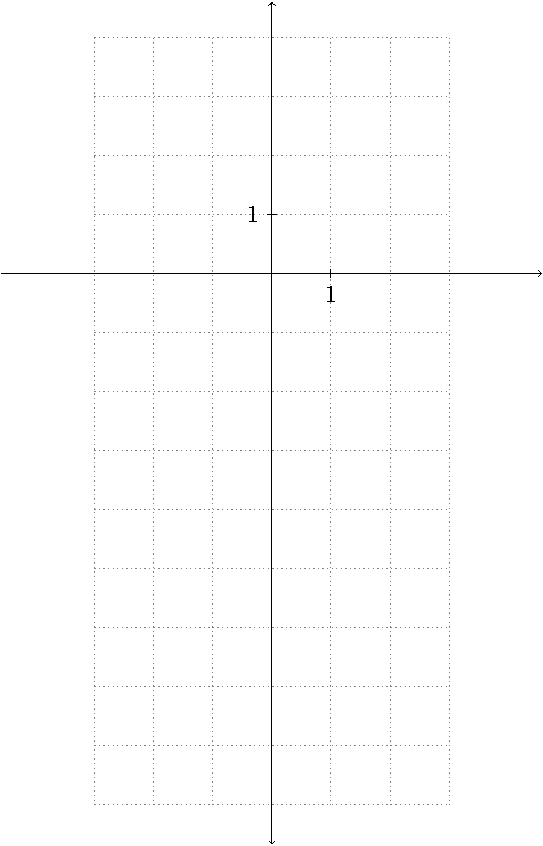
\includegraphics[scale=.85]{Images/plano.pdf}
\end{minipage}\hfill
\begin{minipage}{.45\textwidth}
Espacio para operaciones
\begin{tabular}{|c|c|}
\hline 
$x$ & $f(x)$ \\ 
\hline 
-3 &  \\ 
\hline 
-2 &  \\ 
\hline 
-1 &  \\ 
\hline 
0 &  \\ 
\hline 
1 &  \\ 
\hline 
2 &  \\ 
\hline 
3 &  \\ 
\hline 
\end{tabular} 
\end{minipage}
 \end{enumerate}

\end{document}
